\documentclass{beamer}
\usetheme{Goettingen}
\usepackage{algorithm, algorithmicx}
\title{Exceptional Control Flow}
\author{XD}
\institute{Peking University}
\date{2021}
\newtheorem{rmk}{Remark}
\newcommand{\SubItem}[1]{
    {\setlength\itemindent{15pt} \item[-] #1}
}
\begin{document}

    \frame{\titlepage}
    \begin{frame}{Outline}
        \tableofcontents
    \end{frame}

    \section{Process}
    \begin{frame}{What can a process see?}
        \begin{itemize}
            \item Continuous time
            \item A private memory space
            \item Exclusive use of the CPU
        \end{itemize}
        \only<2->{All the above are just illusions (or abstracts)!}
    \end{frame}
    \section{Exceptions}
    \begin{frame}{Exceptions}
        Comprises Interrupts, Traps, Faults, and Aborts.
    \end{frame}
    \begin{frame}{Interrupt}
        \begin{itemize}
            \item Async: Not caused by any instruction
            \item Hardware triggered: I/O devices, disk controllers and timer chips
            \item Always returns to the next instruction
        \end{itemize}
        
    \end{frame}
    \begin{frame}{Traps and System Calls}
        \begin{itemize}
            \item Intentionally triggered exceptions: ask for more access
            \item Sync: Caused by the current process
            \item Always returns to the next instruction
        \end{itemize}
        From \emph{user mode} to \emph{kernel mode}.
    \end{frame}
    \begin{frame}{Faults}
        \begin{itemize}
            \item Errors that could be correct: Page fault
            \item Sync
            \item Might return to the next instruction
        \end{itemize}
    \end{frame}
    \begin{frame}{Aborts}
        \begin{itemize}
            \item Unsaveable Errors: Memory failed
            \item Sync
            \item Resulting in the termination of the current process
        \end{itemize}
        \begin{rmk}
            Division by zero could (potentially) be saved, but Linux opt to abort the process when happens.
        \end{rmk}
    \end{frame}
    \section{Concurrency}
    \begin{frame}{Concurrency}
        Some of the processes might seem to be run concurrently.
    \end{frame}
    \begin{frame}{Context Switch}
       Context switching allows concurrency to be implemented. Here is an example.
       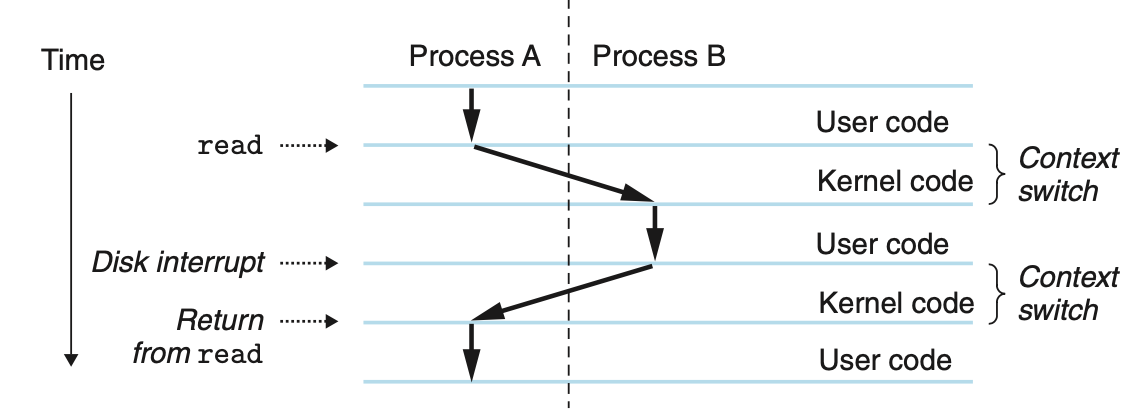
\includegraphics[width=\textwidth]{contextswitching.png}
    \end{frame}

    \section{Private Address}
    \begin{frame}{Private Address Space}
        Also an abstract.
        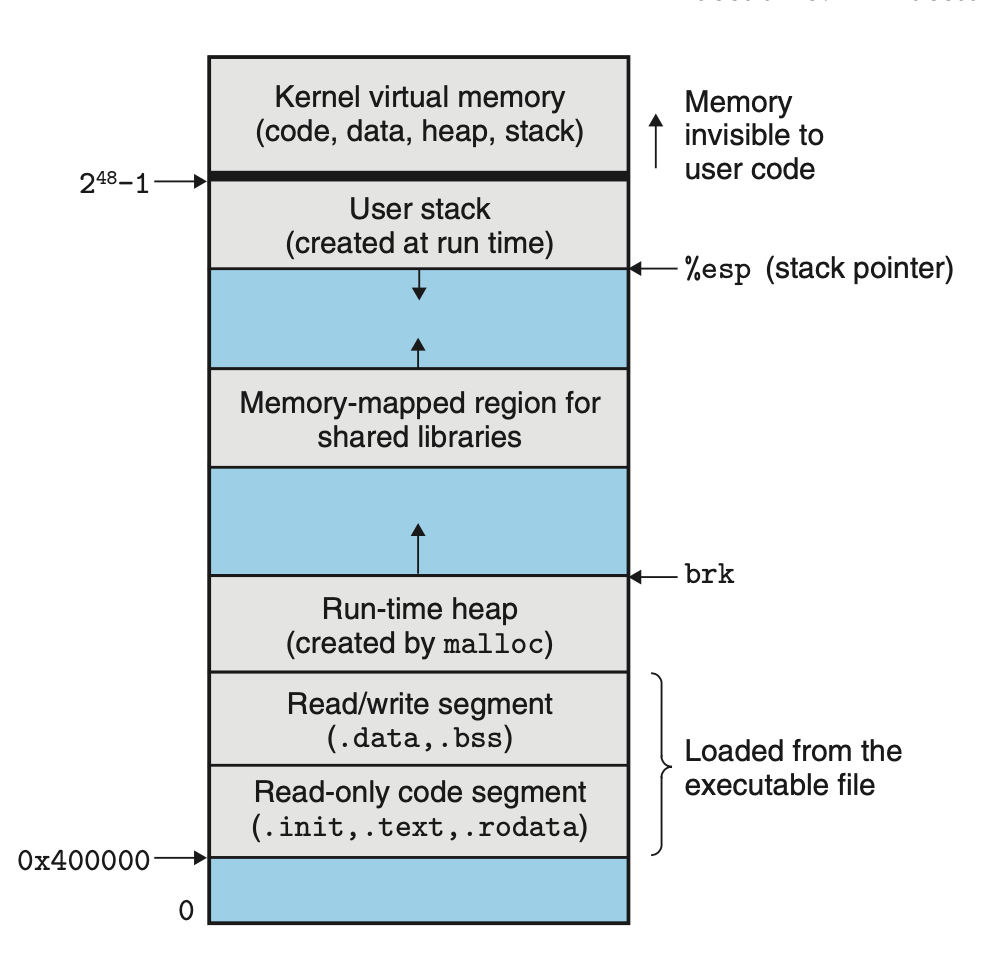
\includegraphics[width=\textwidth]{privatememory.png}
    \end{frame}
    \section{Process Control}
    \begin{frame}{Process Control}
        Process ID(PID)
        \begin{itemize}
            \item getpid(void): return the current PID
            \item getppid(void): return the PID of the parent process
        \end{itemize}
    \end{frame}
    \begin{frame}{Process State}
        \begin{itemize}
            \item Running: Running or going to be run
            \item Stopped: Suspended and won't be scheduled unless receiving SIGCONT
            \item Terminated: Stopped permanently
        \end{itemize}
        \begin{rmk}
            \emph{exit(int status)} could be used to terminate the current process 
        \end{rmk}
    \end{frame}
    \begin{frame}{Fork}
        Fork: opens an \emph{almost identical} child process.\\
        About the child process:
        \begin{itemize}
            \item Start from the return of the fork (Call once, Return twice)
            \item Concurrent execution: no assumption should be made about the execution order
            \item Duplicate but separate address spaces
            \item Shared files: stdout
        \end{itemize}
        Fork() returns 0 for child and the child pid for parent.
    \end{frame}
    \begin{frame}{Fork visualized}
        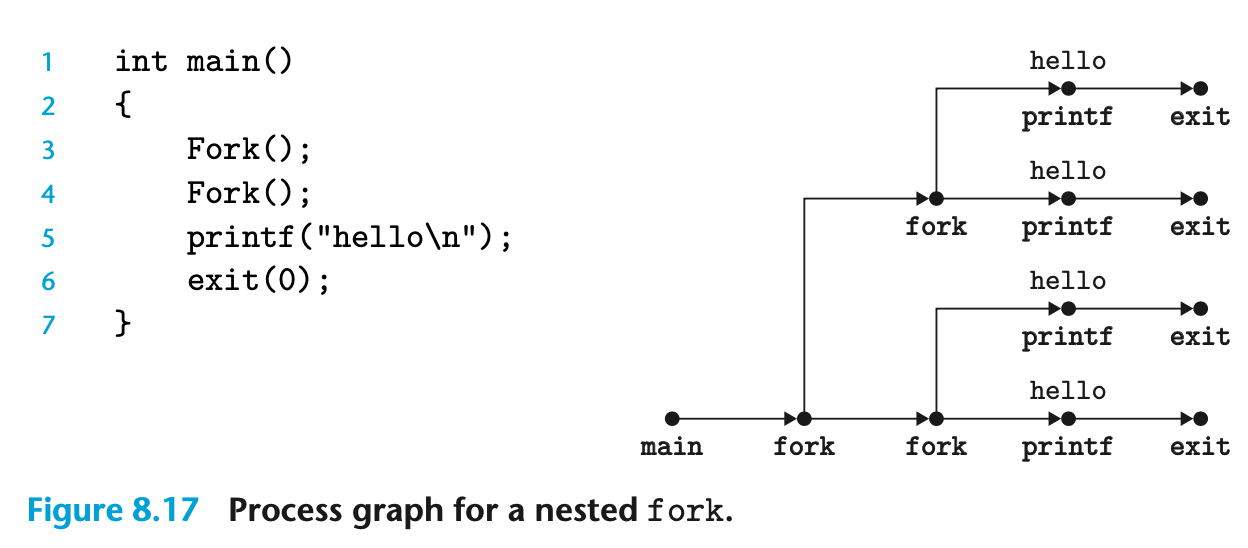
\includegraphics[width=\textwidth]{forkvisualized.png}
    \end{frame}
    \begin{frame}{Reaping Child Processes}
        \begin{definition}
            \textbf{Zombie Process}: terminated yet not reaped\\
        \end{definition}
        Any Orphaned Process would be reaped by init (PID 1, created during the system startup and terminated when shutting off).\\
        To manually ensure a child is reaped, use
        \begin{itemize}
            \item waitpid(int pid, int *statusp, int options)
            \item wait(int *statusp)
        \end{itemize}
    \end{frame}
    \begin{frame}{pid}
        pid determines the wait set of the wait function.\\
        pid > 0: wait set is the child process of which the PID is pid\\
        pid = -1: wait set is all the child processes
    \end{frame}
    \begin{frame}{Option}
        Modify the default behavior of waitpid.
        \begin{itemize}
            \item 0: halt until a child in the wait set terminates
            \item WNOHANG: return immediately if none of the child processes in the wait set has terminated yet
            \item WUNTRACED: halt until a child in the wait set terminates or stops
            \item WCONTINUED: halt until a child in the wait set is terminated or is resumed from SIGCONT
        \end{itemize}
        \begin{rmk}
            Options could be combined, e.g., WNOHANG | WUNTRACED.
        \end{rmk}
    \end{frame}
    \begin{frame}{Quick Quiz \#1}
        What's the equivalent in the form of waitpid(., ., .)  for wait(\&status)?\\
        \only<2->
        {
            \textbf{waitpid(-1, \&status, 0)}
        }
    \end{frame}
    \begin{frame}{Check status}
        Defined in \textbf{wait.h}.\\
    \begin{itemize}
        \item WINEXITED: true if the child terminated normally
        \item WEXITSTATUS: the exit status of a normally terminated child; defined only if WINEXITED is true
        \item WIFSIGNALED: true if the child terminated due to an uncaught signal
        \item WTERMSIG: number of the signal causing the termination of the child; defined only if WINSIGNALED is true
        \item WIFSTOPPED: true if the child causing the return has stopped
        \item WSTOPSIG: number of the signal causing the child to stop; defined only if WIFSTOPPED is true
        \item WIFCONTINUED: true if the child restart on receipt of a SIGCONT
    \end{itemize}
    \end{frame}
    \begin{frame}{Error Condition}
        errno = 
        \begin{itemize}
            \item ECHILD: if the process has no children
            \item EINTR: if waitpid is interrupted by another signal
        \end{itemize}
    \end{frame}
    \begin{frame}{Quick Quiz \#2}
        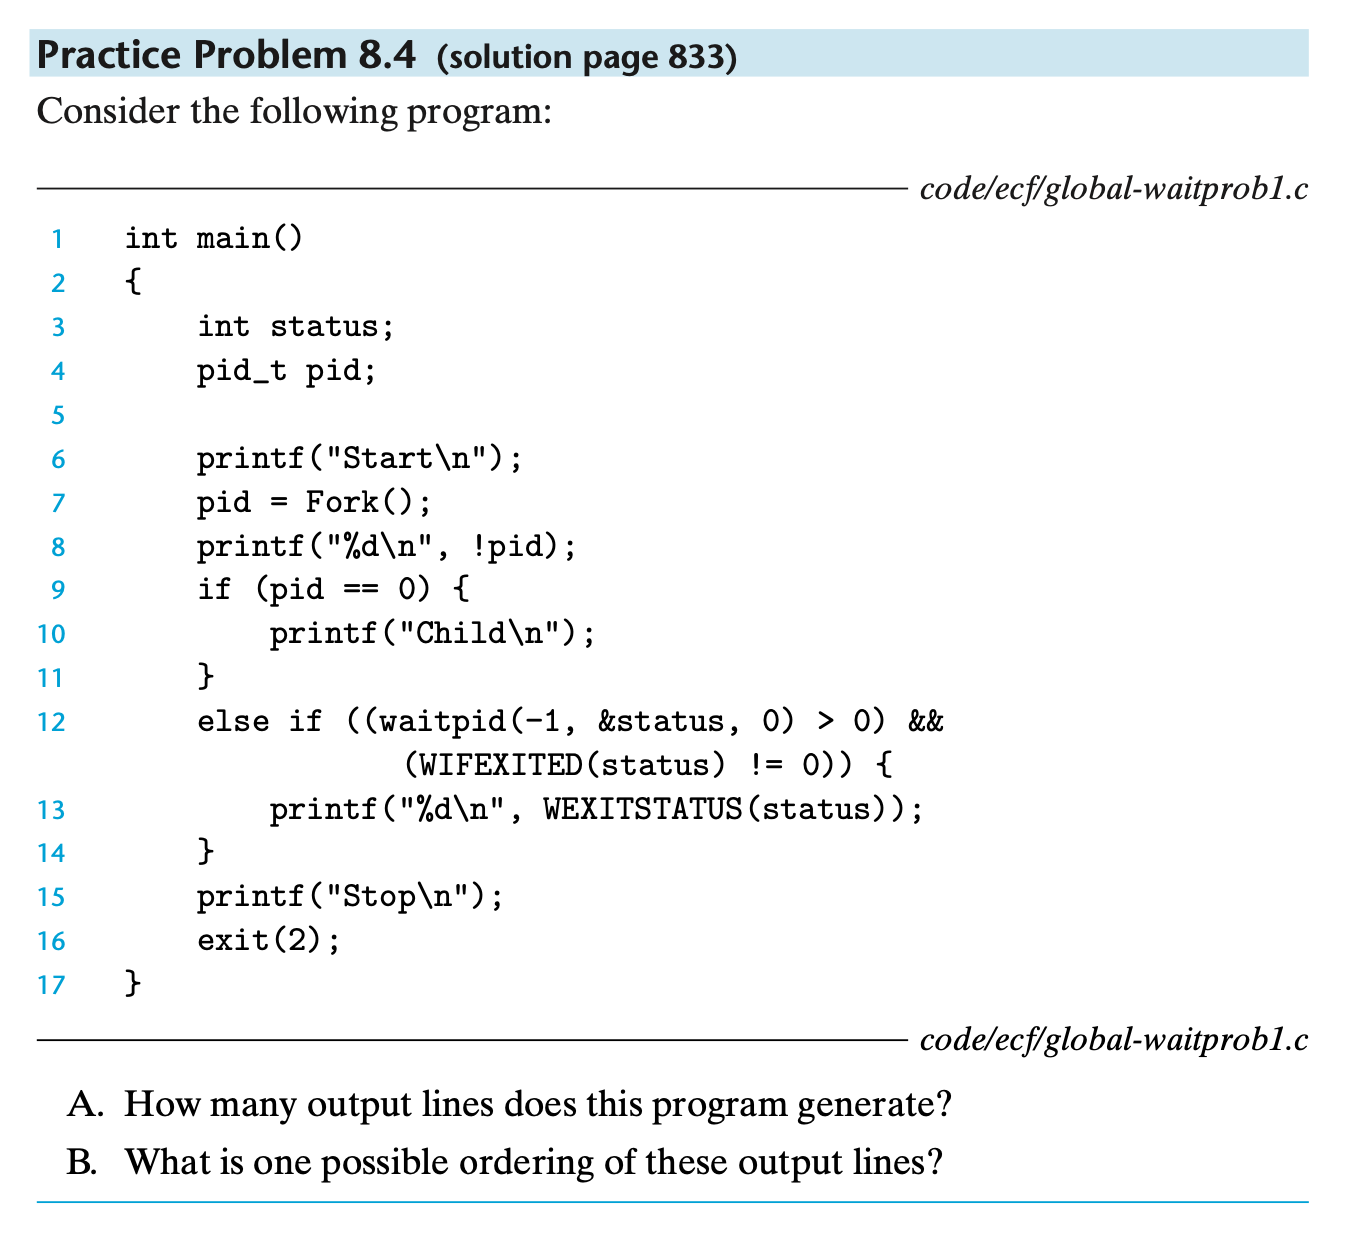
\includegraphics[width=\textwidth]{quiz1.png}
    \end{frame}
    \begin{frame}{Putting processes to sleep}
        \begin{itemize}
            \item sleep(uint s): sleep for s secs
            \item pause(): sleep until waken by a signal
        \end{itemize}
    \end{frame}
    \begin{frame}{Load and Run}
        execve(const char* filename, const char* argv[], const char* envp[])
        \begin{itemize}
            \item filename:
            \item argv: arguments, terminated with NULL
            \item envp: environment, terminated with NULL
        \end{itemize}
        \begin{example}
            argv[] = \{"g++", "-o", "program", "-O2", "xxx.cpp", NULL\}\\
            envp[] = \{"DEBUG=1", NULL\}
        \end{example}
    \end{frame}
    \begin{frame}{Load and Run}
        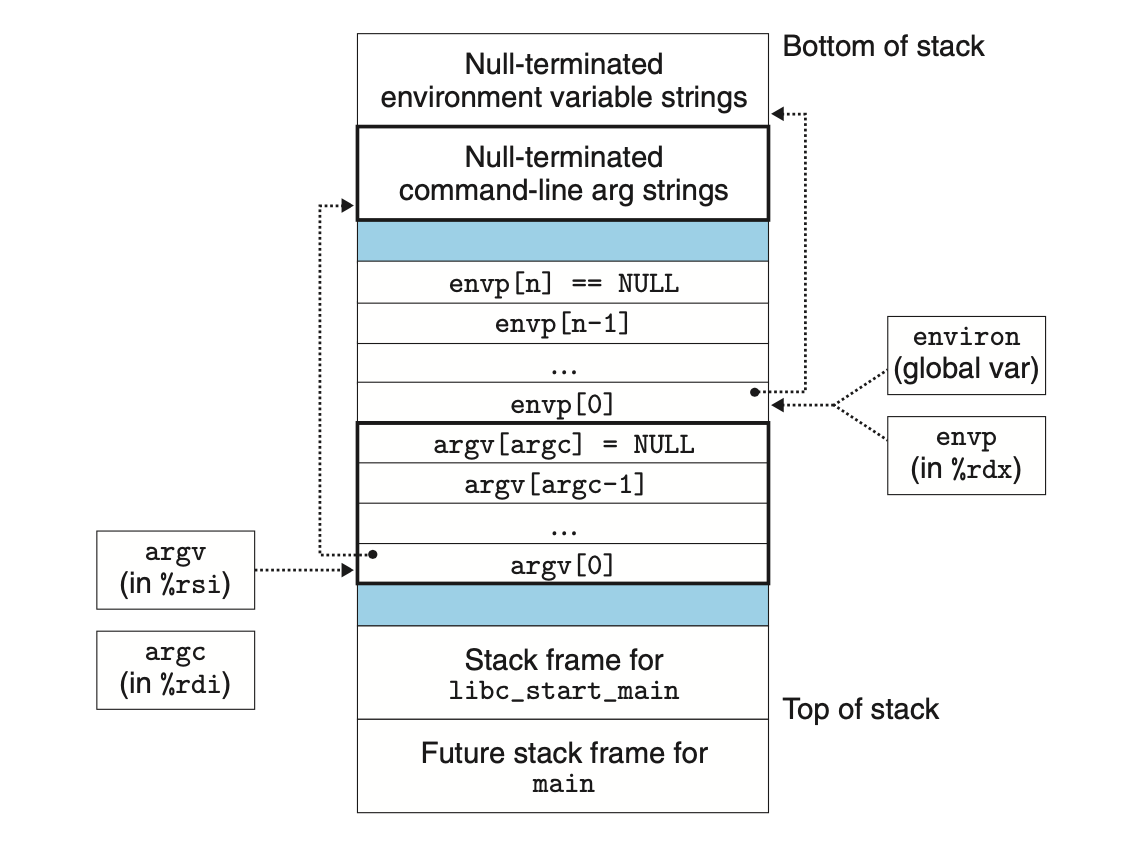
\includegraphics[width=\textwidth]{execvememory.png}
    \end{frame}
    


\end{document}
